\documentclass[../main.tex]{subfiles}

\begin{document}

\chapter{正式踏入编程世界}

对于计算机小白而言,编程的世界可能会显得有些陌生和复杂。要想在这个世界中游刃有余,我们需要掌握的两个重要要素是\textbf{工具}和\textbf{环境}。

工具,指的是我们用来编写和运行程序的东西。包括语言、编辑器等。它们帮助我们更高效地达成我们的目标,例如调试程序、管理项目等。

环境,指的是我们编写和运行代码所依赖的操作系统、编程语言版本以及相关的库和框架。一个良好的编程环境可以大大提高我们的工作效率;同时,我们写出的代码,最终是也要运行在某个环境中的。编程语言本身就是为了让我们能够更方便地与计算机进行交流。

\section{编程语言初探}

\subsection{编程语言的发展简史}

编程语言的发展经历了几个重要阶段:

\begin{itemize}
  \item \textbf{机器语言}:最早的编程语言,直接与计算机硬件对应,使用二进制代码。最早的机器语言是通过拔插电缆实现的,是一个体力活,非常不便。后来改为采用打孔纸带的形式,但仍然非常繁琐和不直观。同时,对于不同的硬件架构,机器语言也不兼容,导致了可移植性差的问题。
  \item \textbf{汇编语言}:在机器语言基础上发展而来,引入了助记符,使得编程更加人性化。同时,汇编语言与特定的指令集相关联,这大大增强了其可移植性,但仍然需要对硬件有一定的了解。汇编语言虽然比机器语言更易读,但仍然需要手动管理内存和硬件资源。
  \item \textbf{高级语言}:高级语言的出现使得编程过程更像说话,而不是在机器上进行什么精确控制硬件的操作,显著增强了其可维护性和可读性;同时同一个高级语言在不同的硬件平台上只需要在对应系统上有一个编译器或解释器就可以运行,这也大大增强了其可移植性。高级语言可以分为两类:
        \begin{itemize}
          \item \textbf{编译型语言}:如C系语言,代码在运行前需要经过编译器转换为机器码,这样可以提高运行效率,但编译过程可能较慢。
          \item \textbf{解释型语言}:如Python,代码在运行时由解释器逐行解释执行,虽然运行速度可能较慢,但开发效率更高,调试更方便。
        \end{itemize}
\end{itemize}

现代的编程语言通常结合了编译型和解释型的优点,提供了更高的抽象层次和更丰富的功能库,使得编程变得更加高效和便捷。微软的.NET系就是一个典型的例子,它提供了一个统一的编程环境,支持多种语言,并且可以在不同的平台上运行。

\subsection{编程语言的特点和选择}

不同的编程语言往往有着自己的特点,选择合适的语言取决于项目需求和个人偏好。

一般情况下,涉及到底层硬件操作、性能要求高的项目,通常会选择编译型语言,如C/C++、Rust等。这些语言提供了对内存和硬件的直接控制,能够实现高效的性能优化;而对于快速开发、原型设计等任务,解释型语言如Python或JavaScript则更为合适。

除了这些通用性语言,还有一些语言能够对特定内容进行极好的支持,例如C\#用于游戏开发,LaTeX用于排版,SQL用于数据库查询,MatLab用于科学计算和数据分析,R用于统计分析等。这些语言通常在特定领域内有着广泛的应用。

不过归根结底,编程语言只是工具。初学者在学习编程的时候,更应该关注的是编程的思想和方法,而不是具体的编程语言。每一门语言都有自己的长处和缺点,在实际使用的时候应该具体情况具体应对。

\section{编程环境的搭建}

编程环境的搭建是编程的第一步。一个良好的编程环境可以大大提高我们的工作效率。

在搭建编程环境之前,我们应当先认识“环境变量”,它是操作系统中存储的变量,用于配置程序运行环境。环境变量可以影响程序的行为,例如指定编译器的路径、设置库文件的搜索路径等。

特别注意:\textbf{系统,尤其是Windows系统是一个很玄学的玩意},有时候需要重启计算机(或者终端)才能使环境变量生效,有时候则不需要。

\subsection{C系编译器及其环境配置}\label{sec:c-install}

对于C语言,有三个最常见的编译器:GCC、Clang和MSVC。它们各有特点,但都能满足大部分初学者的C语言开发的需求。这些编译器通常会与特定的C标准库实现(如GNU的libstdc++、LLVM的libc++或Microsoft的MSVC CRT)配合使用,不同的标准库之间存在细微差异。我们一般建议在Linux上使用GCC,而在Mac上推荐使用Clang。MSVC工具链在Windows上非常流行,但是不跨平台且为闭源软件,有部分程序员可能因此不愿意使用。

Linux和Mac用户可以通过包管理器安装特定的编译器,在暑假课程的《包管理器》一节有讲授,这里不再赘述。

对于Windows用户,有两种方式获得这一编译器:如使用MSVC,则直接下载Visual Studio并安装C++开发模块即可,Visual Studio内置了MSVC工具链;如果使用GCC,则需要通过其他渠道。比起手动下载和配置GCC,我更推荐使用MSYS2或者Cygwin来安装GCC。它们提供了一个完整的Unix环境,免去了在Windows上配置编译器的麻烦。

你需要在\href{https://www.msys2.org/}{MSYS2官网}下载最新的安装包,并按照官网的说明进行安装。安装完成后,你可以通过MSYS2的包管理器pacman来安装GCC。

你可以在MSYS2终端中运行以下命令来安装GCC和GDB(建议使用UCRT64终端,不建议使用逐渐失去支持的32位以及MINGW64环境,也不建议新手使用CLANG64环境,该环境完全使用Clang代替GCC):

\begin{lstlisting}[language=bash]
pacman -S mingw-w64-ucrt-x86_64-gcc
pacman -S mingw-w64-ucrt-x86_64-gdb
\end{lstlisting}

在MSYS2中安装完成后,用户如果想要在Windows终端中使用GCC,则需要设置环境变量,以便在命令行中直接使用编译器命令。

一般情况下,用户需要将MSYS2的bin目录添加到系统的PATH环境变量中。具体步骤如下:

\begin{itemize}
  \item 找到MSYS2的安装目录,通常是\texttt{C:\textbackslash msys64}。
  \item 将\texttt{C:\textbackslash msys64\textbackslash ucrt64\textbackslash bin}添加到系统的PATH环境变量中。(请按照你的实际安装路径进行调整,下同)
  \item 在PowerShell或者CMD中运行以下命令来验证是否配置成功:\texttt{gcc --version}。如果输出了GCC的版本信息,则说明配置成功。
  \item 需要在Windows的PowerShell或者CMD中运行POSIX风格工具时,也可以将下列路径也添加到用户的PATH环境变量中:\texttt{C:\textbackslash msys64\textbackslash usr\textbackslash bin}。但这样具有环境冲突风险,需要注意保证该变量的查找顺序在比ucrt64的bin目录更靠后,以避免冲突。
\end{itemize}

\emph{特别注意:有的同学可能不是按照上述推荐的方式安装GCC的,而是通过其他方式(例如直接下载预编译版本)安装的GCC。如果是这种情况,务必记住GCC和非ASCII字符是死敌,因此请不要将GCC安装在包含非ASCII字符(如汉字、空格)的路径下!(最大的坑可能是你的用户名中包含非ASCII字符,例如汉字!)}

\subsection{虚拟环境及其配置}\label{sec:virtualenv}

开发,尤其是生产类开发有一个重要的原则:不重复造轮子。以Python为例,作为一门流行的编程语言,它拥有丰富的第三方库和框架,可以帮助我们快速实现各种功能,并不需要从零开始开发。

因此,第三方库的安装和管理是开发中非常重要的一部分,而不同的开发往往需要不同的包,或者同一个包的不同版本。这些包有可能会产生冲突,如果用全局环境则会导致依赖混乱。这时,我们引入了虚拟环境,它是解决包冲突的有效手段。

虚拟环境可以理解为一个单独的盒子,包含了特定版本的编译器、解释器和所有依赖的包。用户可以在虚拟环境中自由安装和管理包,而不会影响全局的Python环境。一般有以下几种方法创建虚拟环境:
\begin{itemize}
  \item \textbf{venv}:Python内置的虚拟环境模块,适用于大多数场景。
  \item \textbf{virtualenv}:一个第三方库,提供了更多的功能和灵活性。
  \item \textbf{conda}:Anaconda发行版提供的虚拟环境管理工具,非常简洁高效,逐渐成为目前开发的主流选择。
  \item \textbf{docker}:容器化技术,可以将应用及其所有依赖打包在一个容器中,适用于生产环境,但是由于比较复杂、笨重、资源开销大,一般不推荐用于开发环境。
\end{itemize}

对于学生一般使用的是conda,或者其衍生高速版本mamba。我们的讲述也是以conda为主。

conda有两个发行版,一个是Anaconda,另一个是Miniconda。Anaconda包含了大量的预装包,适合初学者和数据科学家使用;而Miniconda则是一个轻量级的发行版,只包含conda和Python,适合需要自定义环境的用户。我们非常建议使用Miniconda,因为它更轻量,安装速度更快,并且可以根据需要安装所需的包。

特别注意的是,以上两个发行版在Linux和Winget上都难以利用包管理器进行安装。因此,我们一般都是直接从官网下载对应的安装包进行安装。安装完成后,用户需要设置环境变量,以便在命令行中直接使用conda命令。

接下来,因为一些原因,我们应当重启计算机(或者终端),以确保环境变量生效。

然后,我们需要进行终端初始化,例如在Windows上,我们可以使用以下命令:
\begin{lstlisting}[language=bash]
    conda init powershell
\end{lstlisting}

你应该将上述命令替换为你所使用的终端类型,例如在Linux上可以使用\texttt{bash}或\texttt{zsh}。然后你需要重启终端,以使初始化生效。

我们可以创建一个新的虚拟环境,例如:
\begin{lstlisting}[language=bash]
    conda create -n myenv python=3.10
\end{lstlisting}
这样就可以创建一个名为\texttt{myenv}的虚拟环境,并安装Python 3.10的尽可能新的版本。

下面我们需要激活虚拟环境:
\begin{lstlisting}[language=bash]
    conda activate myenv
\end{lstlisting}
这样就进入了虚拟环境,你可以在终端上看到提示符前面有\texttt{(myenv)},表示当前处于\texttt{myenv}虚拟环境中。如没有,可能是终端配置失败或者其他原因,安装OhMyPosh的部分主题也可能会导致这个问题(最大的可能是你的主题没有Python虚拟环境对应的section)。

现在在Python中我们一般流行使用\texttt{pip}来安装包,它从PyPI安装和管理第三方库。现在不流行直接使用conda管理包了。

我们可以使用以下命令安装一个包,例如安装\texttt{Numpy}库:
\begin{lstlisting}[language=bash]
    pip install numpy
\end{lstlisting}
这将会在当前虚拟环境中安装Numpy库,而不会影响全局的Python环境。

如果你需要安装多个包,可以将它们写在一个文件中,例如\texttt{requirements.txt},然后使用以下命令安装:
\begin{lstlisting}[language=bash]
    pip install -r requirements.txt
\end{lstlisting}
以上命令也常用于项目的依赖管理,可以方便地安装和更新项目所需的所有包;同时也可以通过修改\texttt{requirements.txt}文件来管理项目的依赖版本,适宜分发。

\subsection{rust环境搭建}

由于rust工具链依旧依赖着c的工具链所以在安装rust的工具链前,你应该先安装c的工具链,如MSVC、GCC、Clang等(在win上你应该安装MSVC环境,详情见\ref{sec:c-install})。

将会使用rustup来安装rust工具链。

由于众所周知的原因,在安装前你应该换源,如中科大镜像站。在win上请搜索"环境变量",在"系统环境变量"处点击"新建",将如下环境变量添加至系统环境变量中。

\begin{lstlisting}
  变量名             变量值
  RUSTUP_DIST_SERVER https://mirrors.ustc.edu.cn/rust-static
  RUSTUP_UPDATE_ROOT https://mirrors.ustc.edu.cn/rust-static/rustup
\end{lstlisting}

\href{https://rustup.rs/#}{rustup下载}后,就可以点击rustup-init.exe安装了。

在linux上换源方式:将以下设置环境变量的命令放在\texttt{\textasciitilde/.zshrc}(如果你的终端是zsh)或\texttt{\textasciitilde/.bashrc}(如果你的终端是bash)里(这样会在所有终端中生效)

\begin{lstlisting}[language=bash]
  export RUSTUP_DIST_SERVER=https://mirrors.ustc.edu.cn/rust-static
  export RUSTUP_UPDATE_ROOT=https://mirrors.ustc.edu.cn/rust-static/rustup
\end{lstlisting}

然后执行官方脚本来下载rust。

\begin{lstlisting}[language=bash]
  curl --proto '=https' --tlsv1.2 -sSf https://sh.rustup.rs | sh
\end{lstlisting}

\subsection{go环境搭建}

请去\href{https://go.dev/doc/install}{官网下载页面}下载适用于你操作系统的安装包/压缩包。

对于win和mac均是一键安装,对于linux请执行以下命令

\begin{lstlisting}[language=bash]
  sudo rm -rf /usr/local/go && sudo tar -C /usr/local -xzf go1.24.5.linux-amd64.tar.gz
  # 此命令将会删除以前下载的go,并将你下载的压缩包解压并拷贝至/usr/local下(注意将其替换为压缩包的真实路径)
  export PATH=$PATH:/usr/local/go/bin
  # 这行命令建议手动加入~/.zshrc或~/.bashrc,以使环境变量在所有终端生效(说人话:让终端能找到你的go在哪)
  go version
  # 验证go的版本
\end{lstlisting}

\section{选择合适的IDE或者文本编辑器}

IDE(集成开发环境)或者文本编辑器是编程的核心工具之一,用于编写代码、调试和测试等功能。选择合适的IDE或编辑器可以提高编程效率和代码质量。

聪明的懒人宁可使用一天时间来把环境配好来节省以后的时间用来摸鱼,而不是天天花时间来鼓捣环境。

\subsection{选择编辑器}

最Geek的一批程序员最喜欢使用命令行编辑器,例如Vim、Emacs、NeoVim等。这些编辑器通常具有强大的功能和高度的可定制性,适合喜欢命令行操作和自定义配置的用户。但是这些编辑器的使用难度极高,学习曲线陡峭,对于初学者来说极不友好。StackOverflow上的一个非常著名的笑话是“Vim是一个非常强大的编辑器,但是你需要先学会如何退出它”。

\textit{题外话:退出Vim的命令是\texttt{:q},如果你在编辑器中输入了内容并且想要保存,可以使用\texttt{:wq}命令;如果你不想保存,可以使用\texttt{:q!}命令强制退出。}

正课一般推荐以下的几个IDE:C++ IDE是Visual Studio和DevC++,Python IDE是PyCharm。它们各有各的优势,并且有一个最大的共同点:开箱即用,用户并不需要复杂的配置来进行编程。

但是它们的缺点非常明显:Visual Studio(一般简称VS)和PyCharm都非常臃肿,尤其是前者如果安装全家桶需要大量的磁盘空间和内存资源。同时,它们更注重于超大型项目的开发,这一“超大”往往动辄涉及数十万甚至上百万行代码,我们日常学习使用的代码量远远达不到这个级别,只能说是“杀鸡焉用牛刀”。VS的另一个缺点是它实际上专精于Windows平台和微软的.NET生态系统,虽然它也支持C++和Python等语言,但很笨重。至于DevC++,它的功能少得可怜且只支持C/C++。虽然比较适合初学者,但扩展性极差,完全无法满足更复杂的开发需求。

因此,我并不推荐初学阶段就使用这些IDE。从长远来看,使用更加通用的编辑器会更有利于你在编程世界中游刃有余。我们强烈推荐同学们使用Visual Studio Code(VSCode)完成大多数的任务。它是一款轻量级的编辑器,具有良好的扩展性和社区支持,可以满足不同用户的需求。VSCode支持多种编程语言,并且有丰富的插件生态系统,可以根据需要安装各种插件来增强功能。它同时也为调试和版本控制功能添加了GUI,非常适合初学者和中小型项目开发者使用。

除此之外,还有一些语言仅在特定的编辑器中有很好的支持,例如C\#之于Visual Studio,SQL之于DBeaver和DataGrip,Java之于Eclipse等。这些语言通常需要特定的IDE来提供更好的支持和功能,此时再去使用VS Code可能会有些不便。

\subsection{安装VS Code}

我们应该上官网下载安装包进行安装。我们需要安装的是System Installer版本,而不是User Installer版本。因为User Installer版本会将VS Code安装在用户目录下,而System Installer版本会将VS Code安装在系统目录下,这样可以方便地在所有用户之间共享VS Code,并且能够把它直接放在环境变量中。

安装完成后,我们需要设置环境变量,以便在命令行中直接使用code命令。不过如果你在安装时选择了“Add to PATH”选项,则不需要手动设置环境变量。

\subsection{配置VS Code}

VS Code是一个非常灵活的编辑器,可以通过安装插件来增强其功能。常用的插件包括:

\begin{itemize}
  \item \textbf{Python}:提供对Python的支持,包括语法高亮、代码补全、调试等功能。
  \item \textbf{C/C++}:提供对C/C++的支持,包括语法高亮、代码补全、调试等功能。
  \item \textbf{GitLens}:增强版的Git支持,可以更好地查看版本历史和代码变更。
  \item \textbf{Chinese (Simplified) Language Pack for Visual Studio Code}:提供中文界面支持。
\end{itemize}

此外,VS Code还支持多种主题和图标包,可以根据个人喜好进行定制。你可以在VS Code的插件市场中搜索并安装这些插件和主题等。

\subsubsection{在VS Code中配置C/C++}\label{sec:configure-cpp}

如果你使用的是GCC编译器,则需要在VS Code中配置GCC,以便能够编译和运行C/C++代码。可以通过以下步骤进行配置:

\begin{enumerate}
  \item 安装C/C++插件:在VS Code的插件市场中搜索并安装C/C++插件。建议直接安装微软提供的全家桶。
  \item 配置tasks.json文件:在VS Code中创建一个C++文件\texttt{*.cpp}或者\texttt{*.cc},然后随便输入一些什么代码,然后编译之。首次编译C++代码时,VS Code会提示你创建一个\texttt{tasks.json}文件。选择“C/C++: g++.exe 生成活动文件”,这将会在项目根目录下创建一个\texttt{.vscode/tasks.json}文件。(如果你创建的是C文件\texttt{*.c},那么你可以选择“C/C++: gcc.exe 生成活动文件”)
  \item 配置launch.json文件:在VS Code中按下\texttt{F5},选择“C++ (GDB/LLDB)”,然后选择“g++.exe build and debug active file”。这将会在项目根目录下创建一个\texttt{launch.json}文件。(如果没有后一步,可以忽略之。)
\end{enumerate}

如果你并不信任自动生成的配置文件或者需要更多的功能(例如开\texttt{-O2}优化),可以手动创建并修改\texttt{tasks.json}和\texttt{launch.json}文件。这两个文件都应该放在项目根目录下的\texttt{.vscode}文件夹中。

以下是一个简单的\texttt{tasks.json}文件示例(其实就是上面自动生成的那个,按照笔者的计算机环境稍微改了改):

\begin{lstlisting}
{
  "version": "2.0.0",
  "tasks": [
    {
      "label": "C/C++: g++.exe 生成活动文件",
      "type": "shell",
      "command": "g++",
      "args": [
        "-g",
        "${file}",
        "-o",
        "${fileDirname}\\${fileBasenameNoExtension}.exe"
      ],
      "group": {
        "kind": "build",
        "isDefault": true
      },
      "problemMatcher": ["$gcc"],
      "detail": "生成活动文件"
    }
  ]
}
\end{lstlisting}

以下是一个简单的\texttt{launch.json}文件示例:

\begin{lstlisting}
{
  "version": "0.2.0",
  "configurations": [
      {
          "name": "C++ Launch",
          "type": "cppdbg",
          "request": "launch",
          "program": "${fileDirname}\\${fileBasenameNoExtension}.exe",
          "args": [],
          "stopAtEntry": false,
          "cwd": "${workspaceFolder}",
          "environment": [],
          "externalConsole": false,
          "MIMode": "gdb",
          "setupCommands": [
              {
                  "description": "Enable pretty-printing for gdb",
                  "text": "-enable-pretty-printing",
                  "ignoreFailures": true
              }
          ],
          "preLaunchTask": "C/C++: g++.exe 生成活动文件",
          "miDebuggerPath": "C:\\msys64\\ucrt64\\bin\\gdb.exe"
      }
  ]
}
\end{lstlisting}

如不想用JSON文件进行配置,我们还可以使用UI配置相关功能。

在Code中按下\texttt{Ctrl + Shift + P},找到“C/C++: Edit Configurations (UI)”选项。这样就可以通过图形界面来配置C/C++的编译和调试选项。

一般地,我们需要更改以下内容:
\begin{itemize}
  \item 配置名称:默认即可。
  \item 编译器路径:选择你要选用的编译器的路径。该选项一般会自动检测电脑上的编译器。
  \item 编译器参数:留空即可。如需要,可以添加一个\texttt{-O2}或者\texttt{-O3}来开启编译优化,或者添加一个\texttt{-g}来开启调试信息。但是,\texttt{-g}会严重拖慢编译速度,因此建议只在调试时开启。
  \item IntelliSense模式:根据你的系统、编译器、CPU架构选择对应的模式。该选项会为你打开对应的代码补全、语法高亮、错误警示功能。
  \item 包含路径:不用动。
  \item 定义:不用动。
  \item C/C++标准:建议C17和C++17,和PKU线上代码检查的标准一致。其他学校的学生按自己的学校要求来设置,例如14或11。
  \item 高级:一个都不用动。
\end{itemize}

非常闹麻的一点是,调试配置没有UI配置选项,我们还得老老实实地手动编辑\texttt{launch.json}文件。当然默认调试已经够了,如果你不需要更复杂的调试功能,完全可以不修改。


\subsubsection{在VS Code中配置Python}

在VS Code中配置Python非常简单。只需要安装微软提供的三个Python插件,然后在VS Code中打开一个Python文件。

你会在右下角看到一个黄色按钮“选择Python解释器”,点击它可以选择你想要使用的Python解释器。一般情况下,你可以选择“Python 3.x (conda)”或者“Python 3.x (venv)”等选项,这样VS Code就会自动识别你当前的虚拟环境。

当然,我们非常建议同学们趁早熟悉纯命令行运行Python的方式,例如\texttt{python main.py},这样可以更好地理解Python的运行机制,同时也更便于调试(?)。

\subsubsection{在VS Code中配置Rust}

在VS Code中配置Rust比较简单,只需要下载\texttt{rust-analyzer}插件即可。然后用VS Code打开一个空文件夹,打开VS Code的终端(快捷键:\texttt{Ctrl + `}),\texttt{cargo init} 初始化当前的空文件夹。然后在\texttt{src/main.rs}里即可看到\texttt{main}函数的上方有着运行和调试的符号,点击即可运行或调试。

\textit{注意: 初始化后,文件夹下应有着\texttt{Cargo.toml},否则便无法为其提供运行的功能,因为运行是依赖于\texttt{cargo}的。初学者往往会急于创建\texttt{main.rs}而没有用\texttt{cargo init}或\texttt{cargo new dir}来初始化文件夹,然后就会发现\texttt{rust-analyzer}报错\texttt{Failed to discover workspace. Consider adding the Cargo.toml of the workspace to the linkedProjects setting.}}

为了便于调试,我们下载\texttt{codelldb}插件,之后按F5就可以开始调试了。

\subsubsection{在VS Code中配置Go}

安装\texttt{golang.go}插件。然后在终端执行如下命令。(如果你有着足够“好”的网络,那可以不用设置\texttt{GOPROXY})

\begin{lstlisting}[language=bash]
  go env -w GO111MODULE=on # 启用 Go Modules 功能
  go env -w GOPROXY=https://goproxy.cn,direct # 配置代理
  # go env | grep GOPROXY # linux 确认配置
  # go env |findstr "GOPROXY" # windows 确认配置
\end{lstlisting}

下载\textt{go tools}:\textt{Ctrl + Shift + P}打开命令面板输入\textt{Go: Install/Update Tools},选择所有并确定,这将会下载\textt{go tools}。

新建文件夹,用\textt{VS Code}打开此文件夹,新建\texttt{main.go}文件,\texttt{Ctrl + `} 打开终端,输入\textt{go mod init helloworld},编辑\texttt{main.go}

\begin{lstlisting}[language=go]
package main

import (
	"fmt"
)

func main() {
	name := "Go Developers"
	hello := "hello world"
	fmt.Println("Azure for", name, hello)
	hello_world()
}
\end{lstlisting}

按F5即可调试。

\textit{现在Go使用\texttt{go module} 管理依赖,也就是\texttt{go.mod}文件。现在推荐这么做,有些项目可能还在用\texttt{Go Path}来管理,同学遇到了此种项目可自行搜集资料(呜呜,因为我也不知道,等待大佬补充)}

有同学可能发现了,调试的时候并没有输出可执行文件。输出可执行文件:\texttt{go build -o main.exe main.go}, \textt{-o}选项可以指定可执行文件的名字。如果是多文件编译呢?假设源代码均位于src目录下,\texttt{go build src/*.go}。同学们也可了解一下如何交叉编译。

\subsubsection{在VS Code中配置Git}

在VS Code中配置Git同样非常简单。只需要安装Git,并确保Git的可执行文件在系统的PATH环境变量中。然后在VS Code中打开一个Git仓库,VS Code会自动识别并启用Git功能。

\section{美化你的终端}

在Windows上,默认的终端是cmd或者PowerShell,它们的界面比较简陋,不能显示很多信息。为了让终端更美观、更实用,我们可以使用一些终端美化工具,这里我推荐使用\textbf{Oh My Posh}。

\subsection{安装Oh My Posh}

我们建议使用winget来安装Oh My Posh。你可以在PowerShell中运行以下命令来安装:

\begin{lstlisting}[language=bash]
  winget install JanDeDobbeleer.OhMyPosh
\end{lstlisting}

安装完成后,你需要在PowerShell中运行以下命令来初始化Oh My Posh:
\begin{lstlisting}[language=bash]
  oh-my-posh init pwsh
\end{lstlisting}

在配置Oh My Posh的时候,很多的命令涉及到执行脚本。默认情况下,Windows PowerShell会阻止执行脚本以保护系统安全。因此,你需要先修改执行策略来允许执行脚本。在PowerShell中运行以下命令:
\begin{lstlisting}[language=bash]
  Set-ExecutionPolicy -ExecutionPolicy RemoteSigned -Scope CurrentUser
\end{lstlisting}
就可以允许当前用户执行远程签名的脚本。

如果你使用的是其他终端,例如cmd或者Git Bash,你可以在Oh My Posh的\href{https://ohmyposh.dev/docs/installation}{安装文档}中找到相应的安装方法。

\subsection{配置Oh My Posh}

首先,你应该安装OMP推荐使用的字体,例如Nerd Font。这是因为Oh My Posh使用了一些特殊的图标,如果没有合适的字体,可能会导致图标无法正常显示。

你可以在\href{https://www.nerdfonts.com/}{Nerd Fonts官网}下载最新的字体包。安装完成后,你需要在终端中设置字体为Nerd Font,以便能够正确显示Oh My Posh的图标。另一个办法是利用OhMyPosh安装这个字体:
\begin{lstlisting}[language=bash]
  oh-my-posh font install meslo
\end{lstlisting}

安装完成后,你需要在终端中设置字体为Nerd Font。以PowerShell为例,你可以右键点击窗口标题栏,选择“属性”,然后在“字体”选项卡中选择Nerd Font即可。

接下来,你可以在PowerShell中运行命令来设置Oh My Posh的主题了。主题可以在Oh My Posh的\href{https://ohmyposh.dev/docs/themes}{主题文档}中找到。 

\subsection{在VS Code中配置终端}

VS Code内置了终端功能,可以方便地在编辑器中运行命令。终端默认使用系统的命令行工具,例如在Windows上是cmd,在Linux上是bash。

你可以通过快捷键\texttt{Ctrl + `}(反引号)打开终端,也可以通过菜单\texttt{视图 > 终端}来打开。终端打开后,你可以在其中输入命令,和在普通命令行中一样。

如果你希望在VS Code中使用Oh My Posh,只需要把Code的终端字体设置为Nerd Font即可。你可以在VS Code的设置中搜索\texttt{terminal.integrated.fontFamily},然后将其值设置为你安装的Nerd Font的名称,例如\texttt{MesloLGS Nerd Font}。

\section{编写程序的基本素养}

做了这么多操作,我们终于可以编写第一个能跑的程序了。我们将使用C++和Python两个语言来演示怎么书写第一个程序,同时告诉大家编程新手应有的素养。

\subsection{编写你的第一个程序}

由于众所周知的原因,我们的第一个程序通常是“Hello, World!”程序。它的作用是让我们熟悉编程语言的基本语法和编译运行流程,同时也是一个传统。而第二个程序一般往往是写一个加法,让我们熟悉输入输出的基本操作。

\subsubsection{C++}



对于C++,我们可以使用以下代码来编写第一个程序。你可以在VS Code中创建一个新的C++文件,例如\texttt{hello.cpp}(\textbf{该文件的路径不能包含空格和中文!}),然后输入以下代码:

\begin{lstlisting}[language=C++]
#include <iostream>
int main() {
    std::cout << "Hello, World!" << std::endl;
    return 0;
}
\end{lstlisting}

然后如果配置得当,我们就可以通过按下F5键来编译并运行这个程序了。VS Code会自动调用编译器进行编译,并在终端中显示输出结果。如果一切顺利,你应该会看到“Hello, World!”的输出。

在一些极端情况下(例如无GUI环境),你可能需要手动编译和运行程序。可以使用以下命令来编译和运行程序:

\begin{lstlisting}[language=bash]
g++ -o hello hello.cpp
./hello
\end{lstlisting}

请使用类似的方式\textbf{手敲}、编译、运行以下代码:

\begin{lstlisting}[language=C++]
#include <iostream>
int main() {
    int a, b;
    std::cout << "Enter the first integer: ";
    std::cin >> a;
    std::cout << "Enter the second integer: ";
    std::cin >> b;
    std::cout << "Their sum is: " << a + b << std::endl;
    return 0;
}
\end{lstlisting}

\subsubsection{Python}

对于Python,我们同样可以使用以下代码来编写第一个程序:

\begin{lstlisting}[language=Python]
print("Hello, World!")
\end{lstlisting}

同样,如果配置得当,我们就可以通过按下F5键来运行这个程序了。VS Code会自动调用Python解释器运行,并在终端中显示输出结果。同样的,如果希望使用命令行来运行程序,可以使用以下命令:

\begin{lstlisting}[language=bash]
python hello.py
\end{lstlisting}

请使用类似的方式\textbf{手敲}、编译、运行以下代码:

\begin{lstlisting}[language=Python]
a = int(input("Enter the first integer: "))
b = int(input("Enter the second integer: "))
print("Their sum is:", a + b)
\end{lstlisting}

\subsubsection{这两个语言有什么区别?}

可以看到,使用命令行来执行程序的方式有所不同:C++需要两步,但是Python只需要一步。这是因为C++是编译型语言,需要先将源代码编译成可执行文件,然后再运行;而Python是解释型语言,直接运行源代码即可。前者的好处是,一份需要被反复运行的代码只需要编译一次,之后可以反复高效率运行。而后者的好处是,代码修改后可以立即运行,但是需要反复解释执行,运行速度(相对的)非常缓慢。

另一个区别是,C++中,我们可以看到定义a和b之前需要先声明它们的类型,而Python中则不需要。这说明,C++是强类型语言,变量的类型在编译时就确定了;而Python是动态类型语言,变量的类型在运行时才确定。

而这也导致了一个问题:编译器可以识别全部的语法错误和部分的语义错误,因此一份能够编译通过的C++代码,通常代码本身是正确的,但是算法可能因为极端数据出现错误,例如除零等;而Python则无法检查语法错误和语义错误,解释器只会在按顺序运行代码,直到在出现问题的的地方停止。Python 自身的动态类型系统与缺少编译器带来的静态查错系统,使得实际写出来的 Python 代码中经常包含大量的错误。

\emph{在Python的较新版本中引入了“类型注释”,例如\texttt{func(para: int) -> int}。VS Code的Pylance插件能够识别类型注释,并在编辑器中提供有限的类型检查。一些新生代程序员在编写程序时,会使用类型注释来帮助自己检查代码的正确性,防止出现错误。在C++的较新版本中,也引入了“类型推断”,我们可以把部分变量声明为\texttt{auto}类型,例如\texttt{for(auto item : items)},其中\texttt{items}是一个列表。编译器能够自动推断变量的类型,从而减少了代码的冗余。由此可见,编程语言的发展是不断演进的,程序员们不断引入新的特性和语法,以提高代码的可读性和可维护性;同时,我们还可以看到,强类型语言和动态类型语言之间的界限正在逐渐模糊。}

\subsection{学会阅读错误信息}

从上文中我们知道,代码中出现错误是不可避免的一件事情。有时候,我们会犯较为低级的语法错误,此时编辑器会自动指出问题;有时候,我们在只有在代码跑起来的时候才能发现程序错误、不能执行,此时编译器或解释器会给出错误信息,帮助我们定位问题所在;还有一些时候,程序自己运行时并没有因为致命错误而停止运行,但是输出的结果并不是我们期望的,此时我们只能通过调试来解决问题。

例如,以下是C++初学者常见的错误:

\begin{lstlisting}[language=C++]
  #include<iostream>
  using namespace std;
  int mian()
  {
      cout<<"Hello World!"<<endl;
      return 0;
  }
\end{lstlisting}

而它的错误信息是在编译时报出:

\begin{lstlisting}[language=bash]
> g++ example.cpp -o example.exe

ld.exe: *.a(lib64_libmingw32_a-crtexewin.o): in function `main':
C:/.../crtexewin.c:70: undefined reference to `WinMain'
collect2.exe: error: ld returned 1 exit status
\end{lstlisting}

虽然信息略显抽象,但我们还是可以看到很多有用的信息。 ld 是 C++ 中的链接器,再往上看可以发现对 WinMain 的引用是未定义的。这提示我们去看 main 函数,从而发现这里将\texttt{main}函数写成了\texttt{mian},因此链接器无法找到 main 函数,从而引发错误。

而Python给出的错误信息则更为直观,例如以下代码:

\begin{lstlisting}[language=Python]
def calc(numbers):
  total = sum(numbers)
  count = len(numbers)
  return total / count

numbers = [10, 20, 30, 40, 50]
print("Average:", calc(numbers))

numbers.append("60")
print("Updated Average:", calc(numbers))
\end{lstlisting}

其报错是:
\begin{lstlisting}[language=bash]
Average: 30.0
Traceback (most recent call last):
  File "example.py", line 10, in <module>
    print("Updated Average:", calc(numbers))
  File "example.py", line 2, in calc
    total = sum(numbers)
TypeError: unsupported operand type(s) for +: 'int' and 'str'
\end{lstlisting}

可以看到,解释器对第10行和第2行进行了报错。第10行的报错是因为在调用\texttt{calc}函数时,传入的\texttt{numbers}列表中包含了一个字符串“60”,而\texttt{calc}函数期望的是一个数字列表,因此在计算平均值时出现了类型错误(TypeError)。而第2行的报错则是因为在计算总和时,无法将整数和字符串相加。于是我们发现了问题所在:在第9行,我们向\texttt{numbers}列表中添加了一个字符串“60”,而不是一个数字。我们可以通过将其改为\texttt{numbers.append(60)}来解决这个问题。

顺便一提,这段代码在C++这种强类型语言中是无法通过编译的(\texttt{List<int>}类型不能进行append(string)),但 Python 的解释器还是运行代码直到遇到了具体的问题,在输出信息中可以看到第一个 \texttt{print()} 语句仍然被正常地执行。

\subsection{学会调试}\label{subsec:debugging}

调试(技术人一般直接说debug)是我们发现和修复代码中隐藏起来的错误的最有力工具。调试可以帮助我们理解代码的执行流程,从而\textbf{定位}问题所在。

调试有两种手段:静态调试和动态调试。前者一般是通过静态分析工具(例如反汇编器)来分析代码的结构和逻辑,寻找潜在的问题;后者则是通过运行代码并观察其行为来发现问题。静态调试通常用于编译型语言且难度极高,我们不会涉及;而动态调试则适用于所有语言,接下来的内容我们将主要介绍动态调试。

C系有着自己的调试器:GDB(GNU Debugger),它是一个强大的调试工具,可以在命令行中使用。GDB可以让我们逐行执行代码,查看变量的值,设置断点等。VS Code也集成了GDB,可以通过图形界面进行调试。Python也有类似的调试器:PDB(Python Debugger),它同样可以在命令行中使用,也可以通过VS Code进行调试。

纯命令行调试的方式极为困难(尤其是GDB,需要背诵大量的命令),我们在这里不做介绍。然而,VS Code提供了一个非常友好的调试界面,可以通过图形化的方式进行调试。我们可以在代码中设置断点,逐行执行代码,查看变量的值等。这样可以大大提高调试效率。(当然这需要你安装GDB,安装并配置的过程见\ref{sec:configure-cpp}。)

我们调试主要有以下几个手段:打日志、打断点、写测试代码。

\subsubsection{打日志}

打日志是指在代码中添加打印语句,以便在运行时输出某些特定变量的值,进而确定程序的执行流程。这样可以帮助我们理解代码的执行过程,定位问题所在。

新人常常不喜欢这种手段,因为它需要在代码中添加额外的打印语句,很丑陋、不优雅,且会影响代码的可读性和维护性。但是打日志是一个非常有效的调试手段,尤其是在工程量巨大、无法或者很难打断点的情况下。

例如我在调试某数万行的大型项目时,出现断言错误。于是本人在代码中添加了以下打印语句:

\begin{figure}[htbp]
\centering
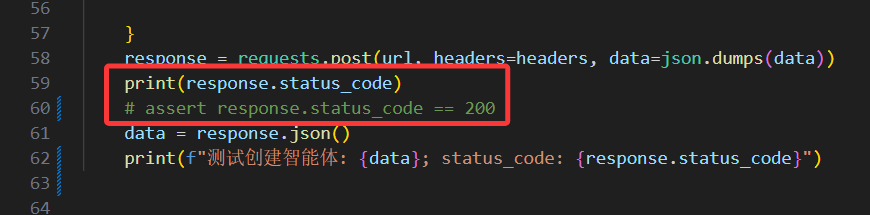
\includegraphics[width=0.8\textwidth]{images/printlog.png}
\caption{打日志的例子}
\end{figure}

这样我就知道了程序在执行到这里的时候,返回的不是预期的200,而是404。于是这让我顺藤摸瓜,排查可能会导致404的原因,最终发现是因为某个API的返回值发生了变化,导致程序无法正常运行。

这是打日志的一个典型例子。通过在代码中添加打印语句,我们可以快速定位问题所在,并进行修复。

\subsubsection{打断点}

在VS Code中,我们可以通过点击行号左侧的空白区域来设置断点。断点是调试过程中非常重要的工具,它可以让代码执行到特定的某行时暂停,从而查看当前的变量值和程序状态。

我们可以逐行执行代码,查看变量的变化,从而定位问题所在。

\begin{figure}[htbp]
\centering
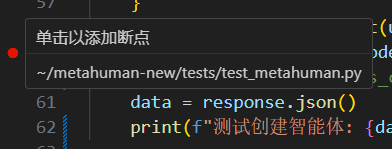
\includegraphics[width=0.8\textwidth]{images/breakpoints.png}
\caption{打断点的例子}
\end{figure}

这样就可以打出一个断点。在调试过程中,当程序执行到断点所在的行时,程序会暂停,我们可以查看当前的变量值和程序状态。我们可以通过单步执行(Step Over)来逐行执行代码,或者通过单步进入(Step Into)来进入函数内部进行调试。对于小型项目或者单文件项目,打断点是一个非常有效的调试手段。

\subsubsection{写测试代码}

写测试代码是指编写一些专门用于测试的代码,以便在运行时验证程序的正确性。测试代码可以帮助我们发现潜在的问题,并确保程序的功能正常。这也是用于较大型项目的调试手段,但是小型项目也可以使用。我们可以在这些测试代码中模拟各种可能出现的情况(包括常规值、边界值、异常值等),从而验证程序的正确性和健壮性。

测试代码通常分为单元测试和集成测试两种。单元测试是对程序的最小可测试单元进行验证,通常是函数或方法;而集成测试则是对多个单元进行组合验证,确保它们能够正常协同工作。

\begin{figure}[htbp]
\centering
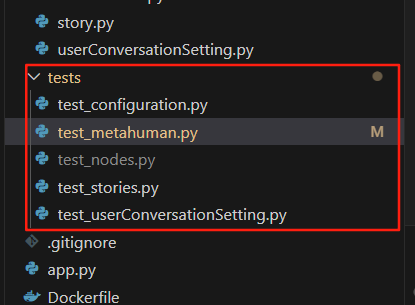
\includegraphics[width=0.8\textwidth]{images/tests.png}
\caption{我为本人实习的项目编写的集成测试}
\end{figure}

\subsubsection{小结}

debug 最重要的一件事是缩小错误出现的范围,为达成这一目的我们通常会跟踪代码的行为,直到发现代码的行为与预期不符。实际上最棘手的情况是,代码只在特定的数据上出现错误,尤其是当我们无法获取程序执行日志的时候。这种情况尤见于我们在POJ上做题的时候:POJ的测试数据是不可见的,只会告诉你结果是WA、RTE还是TLE、MLE。

这时最应该做的是重新审视自己的预期(以及 OJ 题的题面),寻找是否遗漏了什么约束条件或关键信息。一份貌似运行正常的代码很有可能会在边界条件或复杂数据的情况下出问题,可以尝试手写一些处于边界条件之下的数据,或编写一个数据生成器来生成更复杂的数据。实在手足无措时,休息一下放空大脑也是很好的选择。实在走投无路之时,摇人求助也不是什么大不了的事情。debug 很可能会占用比编写代码更多的时间和精力,保持良好的心态才是 debug 的关键。

\end{document}